\documentclass[hyperref={pdfpagelabels=false}]{beamer}
\usepackage{lmodern}
\usetheme{CambridgeUS}
\definecolor{SURFsara-gray}{HTML}{f1edf4}
\definecolor{SURFsara-green}{HTML}{168545}
\setbeamercolor{palette primary}{use=structure,fg=SURFsara-green,bg=SURFsara-gray}
\setbeamercolor{palette secondary}{use=structure,fg=SURFsara-green,bg=SURFsara-gray}
\setbeamercolor{palette tertiary}{use=structure,fg=SURFsara-gray,bg=SURFsara-green}
\setbeamercolor{structure}{fg=SURFsara-green,bg=SURFsara-gray}
\setbeamercolor{title}{fg=SURFsara-green}
\setbeamercolor{frametitle}{fg=SURFsara-green}
\setbeamertemplate{title page}[default][]
\newcommand\blfootnote[1]{%
   \begingroup
   \renewcommand\thefootnote{}\footnote{#1}%
   \addtocounter{footnote}{-1}%
   \endgroup
}

\title{Parallelization}
\subtitle{}
\author{Jeroen Engelberts}
\institute[SURFsara]{PhD Theoritical Chemistry\par Consultant for Cartesius and Lisa}
\date{\today}


\begin{document}
    \logo{
\includegraphics[scale=0.015]{images/SURFsara_logo.png}}
    \begin{frame}
        \titlepage
    \end{frame}

    \AtBeginSection[]{
        \begin{frame}
            \begin{beamercolorbox}[center]{title}
                \usebeamerfont{title}\insertsectionhead\par%
            \end{beamercolorbox}
        \end{frame}
    }


    \begin{frame}
        \frametitle{Table of contents}
        \tableofcontents
    \end{frame} 


    \section{Concepts} 
    \subsection{Serial}
    \begin{frame}
        \frametitle{Serial}
        \begin{center}
            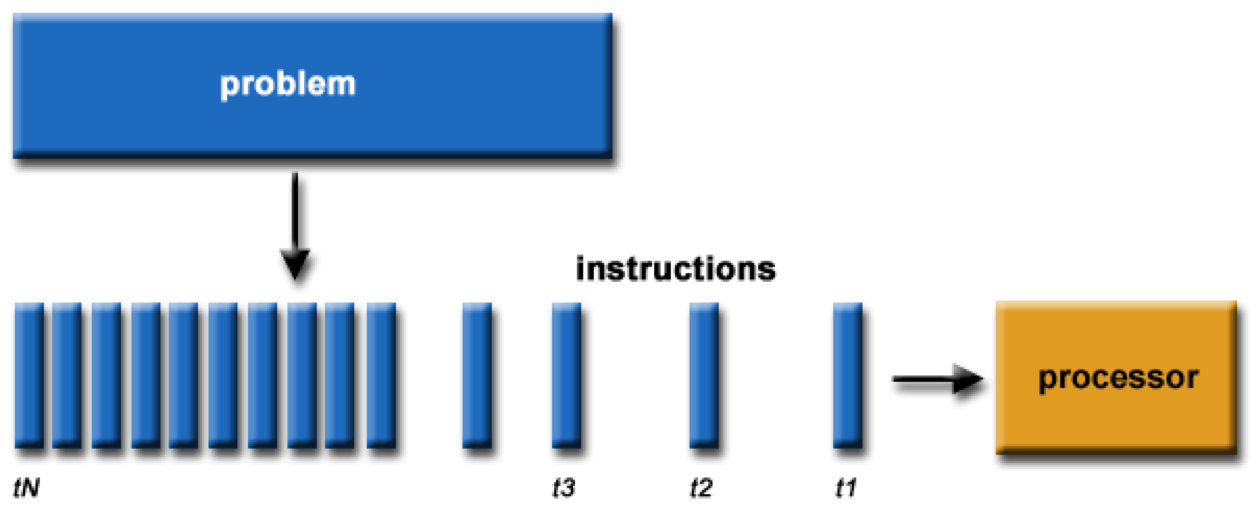
\includegraphics[scale=0.4]{images/serial.png}
            \blfootnote{\tiny{Author: Blaise Barney, Lawrence Livemore National Laboratory}}
        \end{center}
    \end{frame}
    
    \subsection{Parallel}
    \begin{frame}{Parallel}
        \frametitle{Parallel}
        \begin{center}
            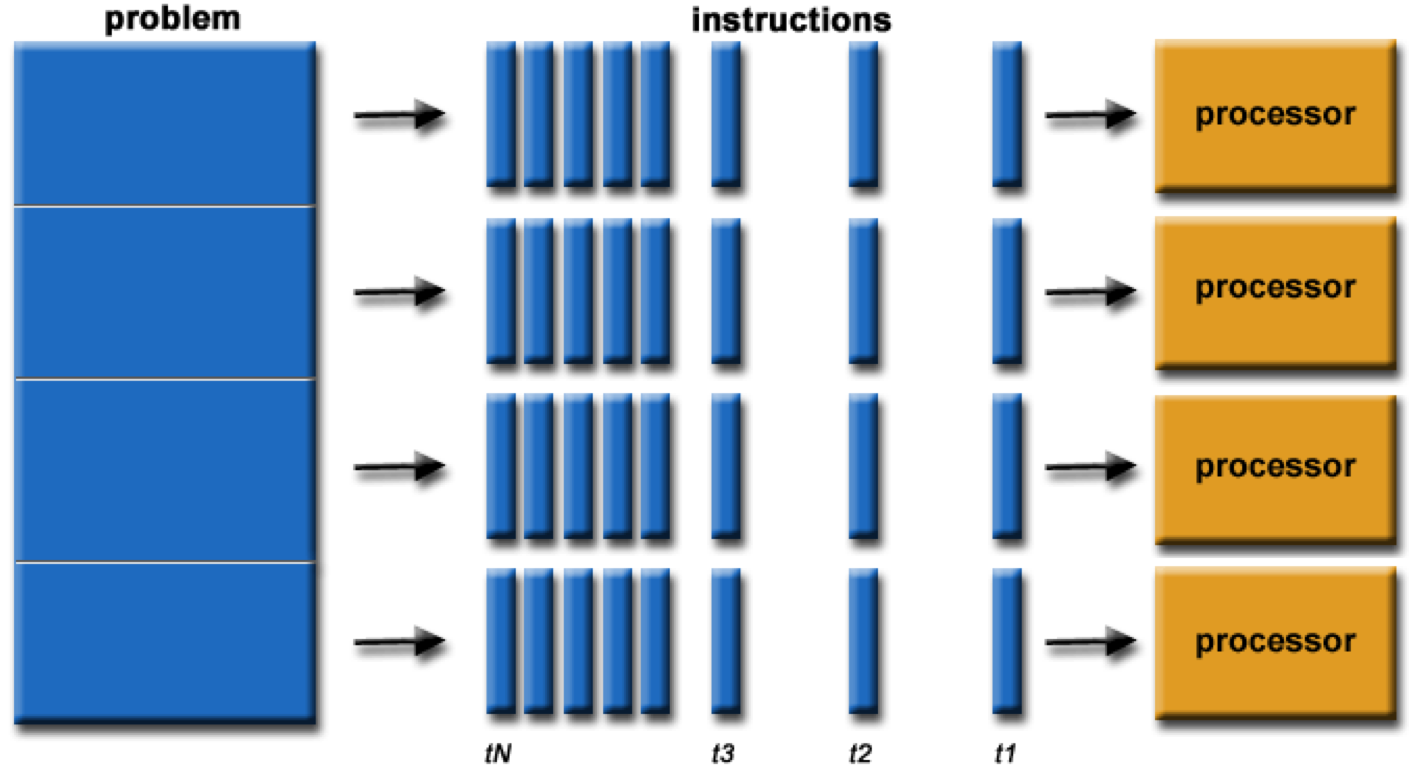
\includegraphics[scale=0.4]{images/parallel.png}
            \blfootnote{\tiny{Author: Blaise Barney, Lawrence Livemore National Laboratory}}
        \end{center}
    \end{frame}
    
    \subsection{Parallelization Methods}
    \begin{frame}{Shared Memory}
        \frametitle{Shared Memory}
        \begin{center}
            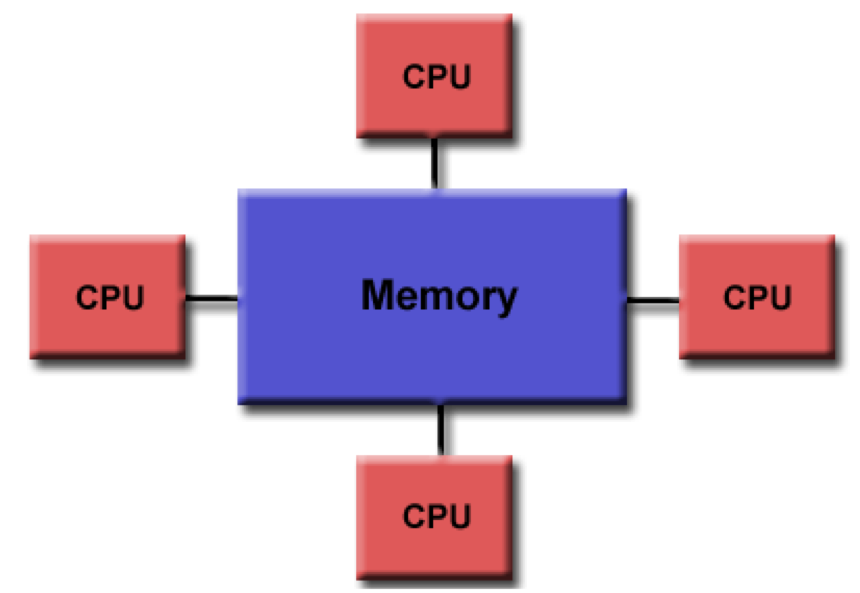
\includegraphics[scale=0.4]{images/shared_memory.png}
            \blfootnote{\tiny{Author: Blaise Barney, Lawrence Livemore National Laboratory}}
        \end{center}
    \end{frame}
    
    \begin{frame}{Distributed Memory}
        \frametitle{Distributed Memory}
        \begin{center}
            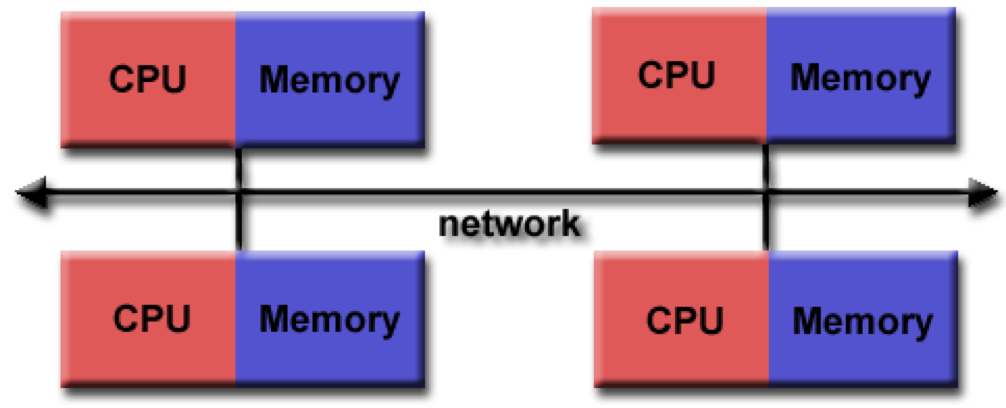
\includegraphics[scale=0.4]{images/distributed_memory.png}
            \blfootnote{\tiny{Author: Blaise Barney, Lawrence Livemore National Laboratory}}
        \end{center}
    \end{frame}
    
    \begin{frame}{Hybrid: Shared and Distributed Memory}
        \frametitle{Hybrid: Shared and Distributed Memory}
        \begin{center}
            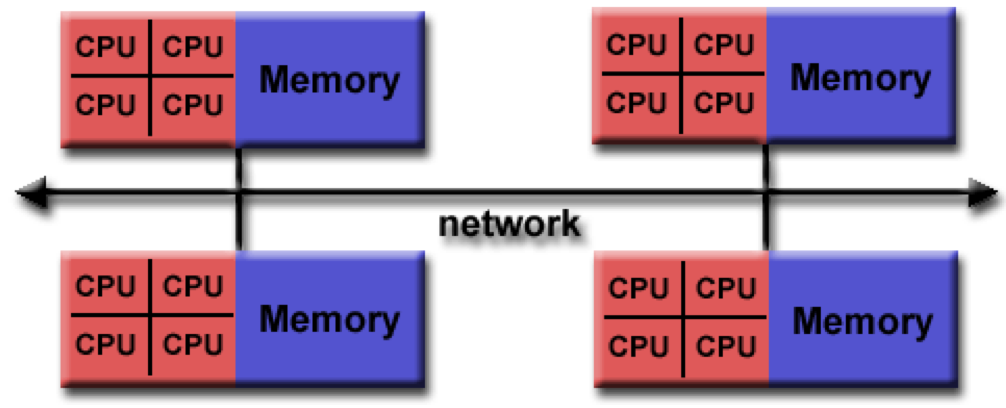
\includegraphics[scale=0.4]{images/hybrid.png}
            \blfootnote{\tiny{Author: Blaise Barney, Lawrence Livemore National Laboratory}}
        \end{center}
    \end{frame}

    \section{OpenMP} 
    \subsection{Description}
    \begin{frame}
        \frametitle{OpenMP - Description}
        \begin{itemize}
            \item Standard library, present in mostly all modern C and Fortran compilers 
            \item Set $OMP\_NUM\_THREADS=n$, n a positive number
            \item Can be run as any other program
            \item Code can be parallelized per loop
            \item Can scale up to one node (only)  
        \end{itemize} 
    \end{frame}

    \subsection{Example}
    \begin{frame}
        \frametitle{OpenMP - Example}
        \begin{itemize}
            \item Introduction to  \LaTeX{}  
            \item Course 2 
            \item Termpapers and presentations with \LaTeX{}  
            \item Beamer class
        \end{itemize} 
    \end{frame}

    \section{MPI} 
    \subsection{Description}
    \begin{frame}
        \frametitle{MPI - Description}
        \begin{itemize}
            \item Additional library, needs to be installed separately  
            \item Program needs to be run with a wrapper: mpirun, mpiexec or srun
            \item Existing code needs a rewrite,
            \item A new program needs to be designed parallel from the start 
            \item Can scale up beyond one node
        \end{itemize} 
    \end{frame}

    \subsection{Example}
    \begin{frame}
        \frametitle{MPI - Example}
        \begin{itemize}
            \item Introduction to  \LaTeX{}  
            \item Course 2 
            \item Termpapers and presentations with \LaTeX{}  
            \item Beamer class
        \end{itemize} 
    \end{frame}

    \section{Wrap-up}
    \subsection{Questions and Answers}
    \begin{frame}
        \frametitle{Thank you for your attention!}
        \begin{center}
           
\includegraphics[scale=0.5]{images/qa.png}
        \end{center} 
    \end{frame}

\end{document}